%!TEX encoding = UTF-8 Unicode

\section{関連研究}

\subsection{緒言}
本章では関連研究のついて述べる.はじめに一般的なHPCシステムの利用方法,続いてOpenOnDemandと呼ばれるインタフェース,最後に現行のインタフェースにおけるの課題を述べる.

\subsection{HPCシステム利用方法}
HPCシステムとは,スーパコンピュータやコンピュータクラスタの能力を利用して,ほかのコンピュータを遥かに凌ぐ速度で計算課題(ジョブ)を処理し,実行するシステムを指す.このようなコンピューティング能力の集約によって,さまざまな科学分野において他の方法では対処できない大きな課題を解決できる.実際に,平均的なデスクトップコンピューターは毎秒数十億の計算を実行できる.これは,人間が複雑な計算を行うことができるスピードに比べれば,素晴らしい数字である.しかし,HPCシステムは,1秒に数千兆の計算を実行することができるため,大規模な課題に対してはより適しているといえる.\par
一般的にHPCシステムの利用の流れを図\ref{fig4}に示す.HPCシステムは数種類のサーバやデータベースから構成される.ジョブを実行するために計算を行う計算サーバ(ワーカーノード),ワーカーノードを管理するためのジョブスケジューラが搭載されたジョブ管理サーバ(マスターノード),ユーザ情報が保存されたデータベースと連携してログイン情報の管理やユーザリクエストの受け渡しを行うログイン用サーバ,実行するジョブのファイルなどが保存されたファイルサーバなどがシステムの構成例である.ユーザはログイン用サーバが取り扱うユーザ情報を用いてHPCシステムにログインする.ユーザはログインサーバを通じてマスターノードにジョブの実行を依頼する.マスターノードは依頼されたジョブのファイル情報などをファイルサーバと連携して受け渡しを行い,ワーカーノードにジョブの実行を依頼する\par
ユーザは利用したいクラスタを遠隔で操作するために自身のコンピュータからユーザ情報を用いて鍵の登録を行った後,ログイン用サーバにssh接続する.そして,ユーザは利用するジョブスケジューラの種類に応じた形式でジョブスクリプトを作成する.その後,与えられたコマンドを用いてジョブを投入を行う.マスターノードのジョブスケジューラが実行するジョブの管理を行い,ワーカーノードはマスターノードの命令に従ってジョブの実行を行う.実行が終了したジョブは標準出力とエラーファイルが出力され,ジョブの実行結果を確認することができる.\par

\begin{figure}[tb]
    \centering
    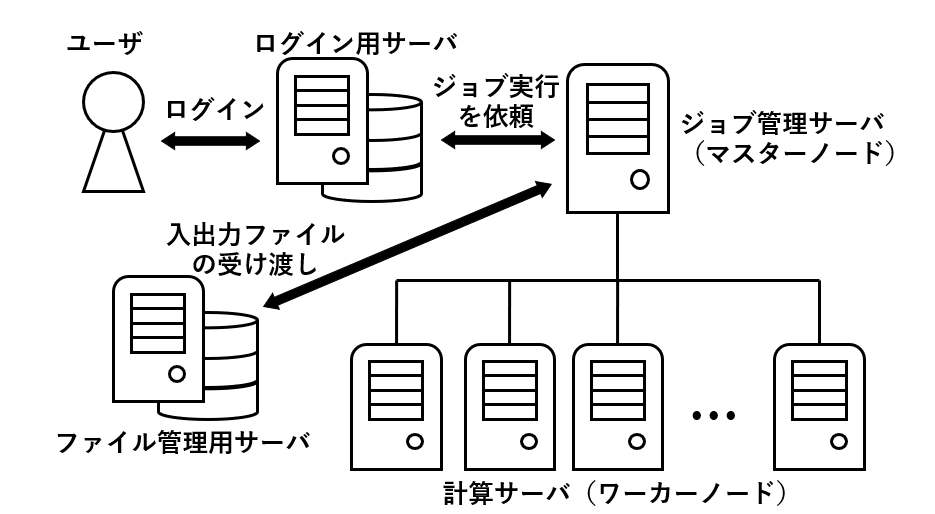
\includegraphics[width=100mm]{./fig/HPCsystem.png}
    \caption{一般的なHPCシステムの模式図}
    \label{fig4}
\end{figure}

\subsection{Open OnDemand}
代表的な関連研究として,Open OnDemand(OOD)とその機能や設計構成を紹介する\cite{cite2}\cite{cite3}.OODは米国オハイオ・スーパーコンピューティングセンターが開発したオープンソースソフトウェアであり,ウェブインタフェースを介してHPCシステムを利用できる環境を提供する.ユーザはウェブブラウザ上でHPCクラスタを簡単に操作することができ,プラグインやほかのソフトウェアのインストールや設定は不要である.また,リモートデスクトップやjupyternotebook,VSCodeなどのグラフィカルな対話的操作もウェブブラウザ上から利用することができる.OODは世界的に使われている様々なジョブスケジューラ(PBS Pro,Slurm,Grid Engine,Torque,LSFなど)に対応しているためシステム間の利用方法の差異を隠蔽している.\par
初めに,OODの機能について説明する.OODは,図\ref{dashboard}に示すダッシュボードとユーザのディレクトリを管理するFilesアプリ,ジョブの管理を行うjobsアプリ,シェルの操作を行うClustersアプリ,開発者が任意の追加アプリを導入することができるinteractiveappsから構成される.図\ref{homedirectory}に示すfilesからはユーザのディレクトリをグラフィカルに操作することができ,ファイルやディレクトリの削除追加編集なども容易に行うことができる.図\ref{activejobs}にはジョブの状態確認を行うActive Jobs画面を示す.ユーザは投入したジョブの状態をリアルタイムで確認することができる.図\ref{jobcomposer}にはJobsのジョブ管理を行うJobComposerの画面を示す.ユーザはジョブの作成と投入削除などをすべてこの画面から行うことができる.図\ref{shell}には,shell画面を示す.ユーザは連携したHPCクラスタのシェルをウェブブラウザ上から操作することができる.このように,OODは様々なアプリケーションと連携してHPCユーザの利用支援を行っている.\par
続いて,OODのの設計について説明する.OODは現在多様なジョブスケジューラに対応しているが,各ジョブスケジューラへの対応はadaptersディレクトリ下に配置される.指定したジョブスケジューラに対応するために,各々でAdapterクラスのサブクラスが宣言され,内部ではジョブスケジューラに合わせてジョブの投入を行うメソッドやジョブの削除を行うメソッド,ジョブの情報を取得するメソッドが再定義されている.対応するAdaoterファイルを呼び出して参照することでOODは多様なジョブスケジューラに対応することができている.\par

\begin{figure}[tb]
    \centering
    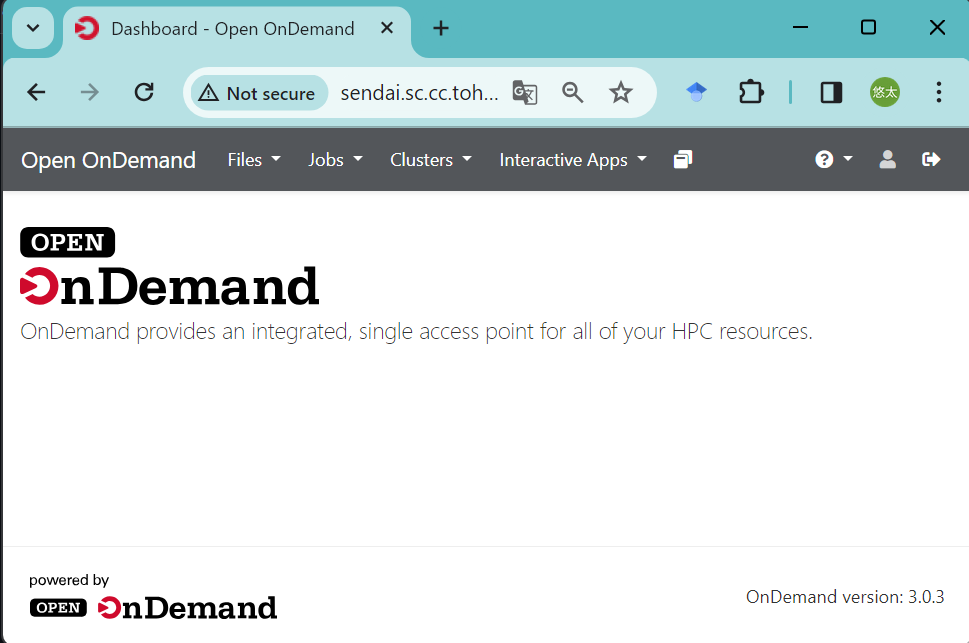
\includegraphics[width=100mm]{./fig/dashboard.png}
    \caption{ダッシュボード画面}
    \label{dashboard}
\end{figure}

\begin{figure}[tb]
    \centering
    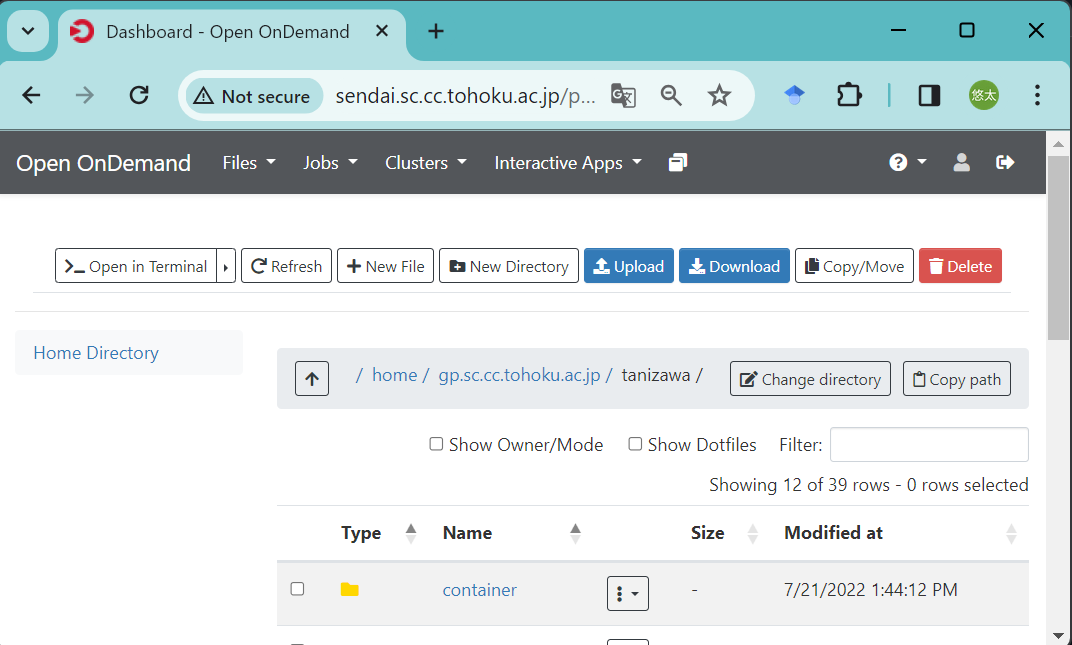
\includegraphics[width=100mm]{./fig/homedirectory.png}
    \caption{ホームディレクトリ画面}
    \label{homedirectory}
\end{figure}

\begin{figure}[tb]
    \centering
    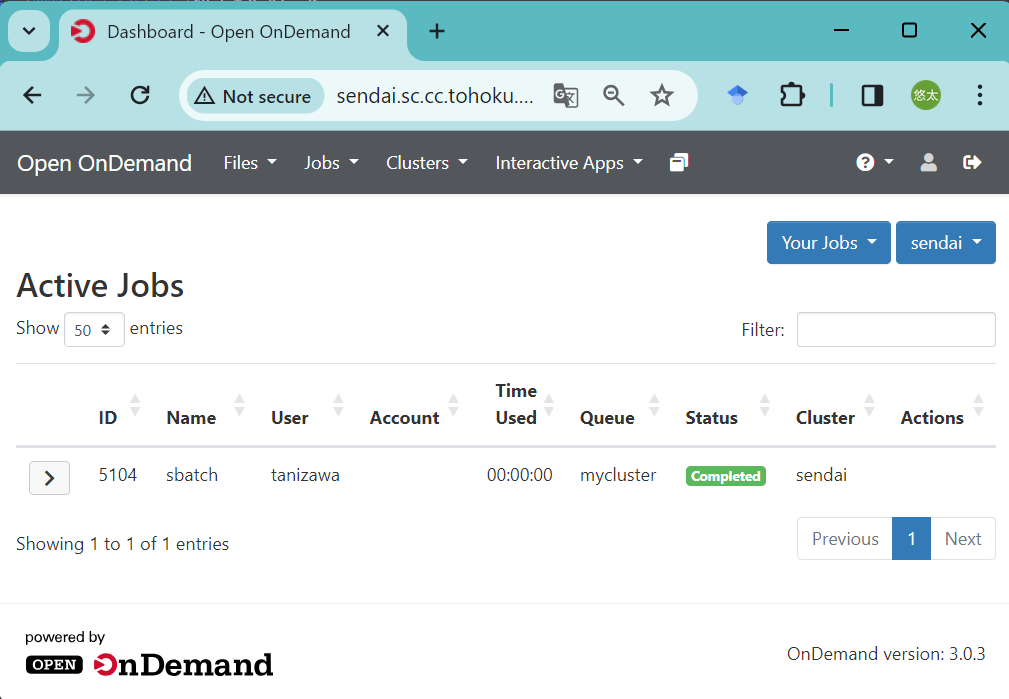
\includegraphics[width=100mm]{./fig/activejobs.png}
    \caption{ジョブ状態確認画面}
    \label{activejobs}
\end{figure}


\begin{figure}[tb]
    \centering
    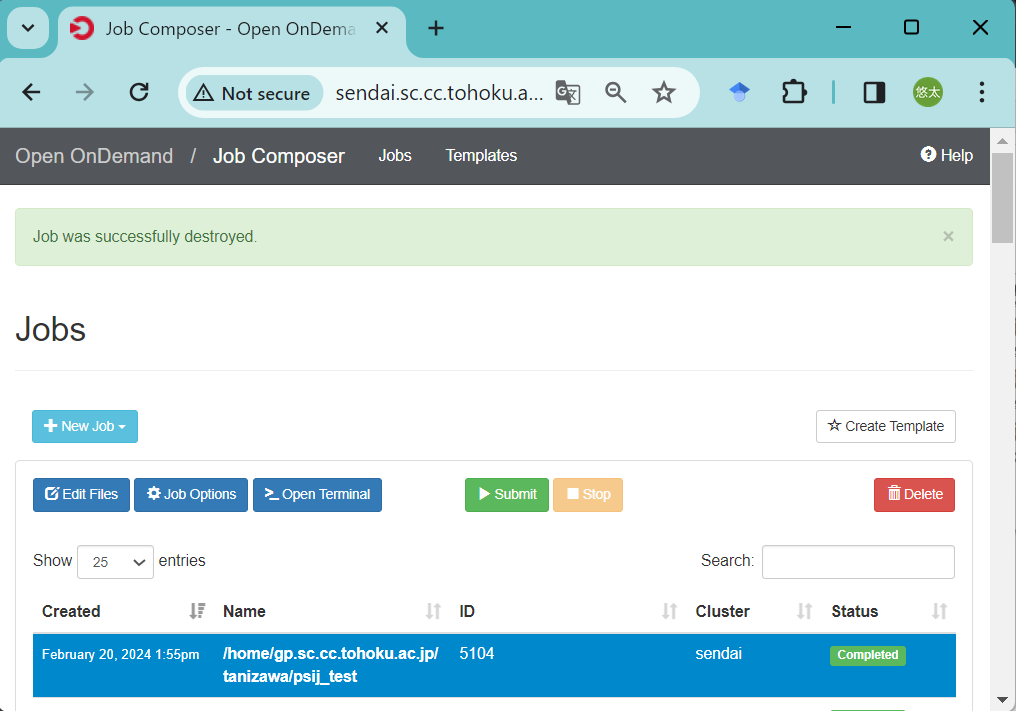
\includegraphics[width=100mm]{./fig/jobcomposer.png}
    \caption{ジョブ管理画面}
    \label{jobcomposer}
\end{figure}

\begin{figure}[tb]
    \centering
    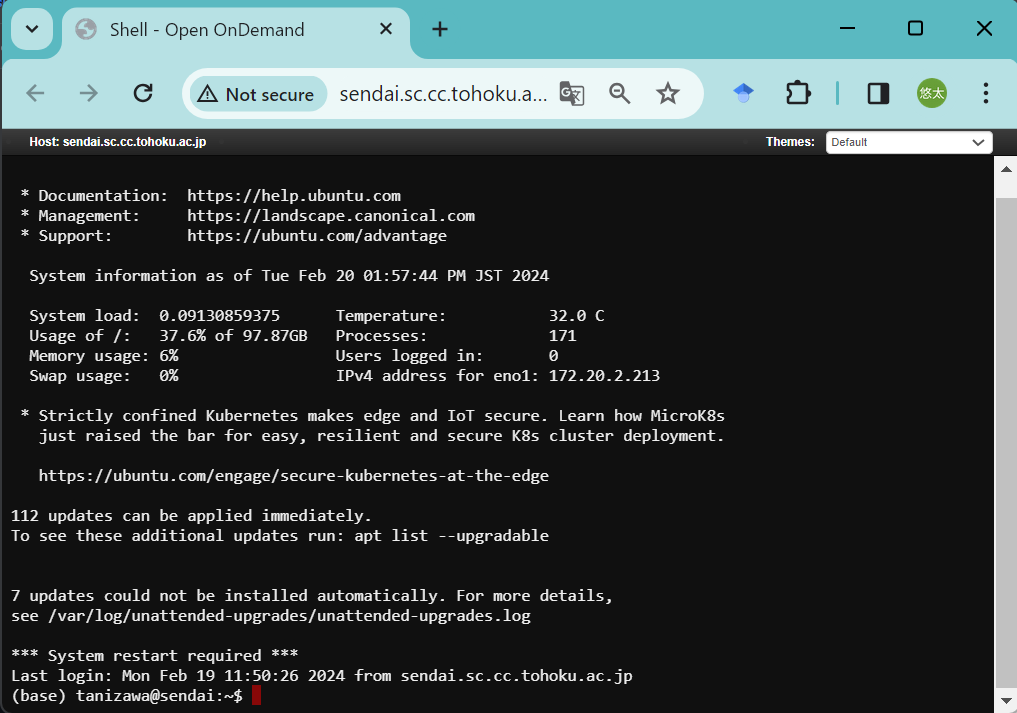
\includegraphics[width=100mm]{./fig/shell.png}
    \caption{シェル画面}
    \label{shell}
\end{figure}

\subsection{現行のウェブインタフェースにおける課題}
現行のウェブインタフェースにおける課題について説明する.国内でのウェブインタフェースの実装事例として,スーパコンピュータ富岳でのOODの実装が挙げられる.OODは汎用的なツールであるが,富岳で用いられているジョブスケジューラ(Fujitsu Technical Computing Suite, Fujitsu-TCS)に対応していなかったことから,中尾らはOODをFujitsu-TCS向けに改修した事例を報告している\cite{cite4}.Fujitsu-TCSに対応するために,新たなAdapterファイルを作成し,Fujitsu-TCS用のメソッドを再定義することによりOODはFujitsu-TCSへの対応を行うが,このような改修方法はシステムの基幹部分を直接改修しなければいけないため,慎重に作業を行う必要がある.このように,ほかにも様々なジョブスケジューラが存在し,今後も登場することを考えると,ジョブスケジューラがの種類が増えるごとにOOD本体を直接改修する方法では問題があるといえる.\par


\subsection{結言}
本章では,関連研究について述べた.はじめに一般的なHPCシステムの利用方法について説明した.その後,Open OnDemandと呼ばれるインタフェースについてその機能と設計について説明した.最後に,現行のインタフェースについて,国内でのOODの実装例を参考にして課題点を述べた.次章では,本章で述べた現行のウェブインタフェースにおける課題である保守性を考慮した手法を提案し,その実装を行う.\par